% !TeX TXS-program:compile = txs:///lualatex

\documentclass[a4paper,11pt]{article}
\usepackage[breakable]{cp-base} %avec options possibles parmi breakable (tcbox), sujetl (exos),  (pour faire "comme avant"), etc...
\graphicspath{{./graphics/}}
%variables
\donnees[%
	typedoc=CHAPITRE~,
	numdoc=8,
	classe=1\up{ère} 2M2,
	matiere={[SPÉ.MATHS]},
	annee=2021,
	titre={Fonctions dérivées}
	]

%formatage
\author{Pierquet}
\title{\nomfichier}
\hypersetup{%
	pdfauthor={Pierquet},pdftitle={\nomfichier},allbordercolors=white,pdfborder=0 0 0,pdfstartview=FitH}
%divers
\lhead{\entete{\matiere}}
\chead{\entete{\lycee}}
\rhead{\entete{\classe{} - Chapitre \thepart}}
\lfoot{\pied{\matiere}}
\cfoot{\logolycee{}}
\rfoot{\pied{\numeropagetot}}

\begin{document}

\pagestyle{fancy}

\part{CH08 - Fonctions dérivées}

\section{Rappels}

\begin{cprop}[ - Rappel]
Une fonction est $f$ est \textbf{dérivable en $a$} si le taux d'accroissement $\frac{f(a+h)-f(a)}{h}$ admet une limite finie lorsque $h$ tend vers 0, cette limite étant le \textbf{nombre dérivé} $f'(a)$.

Graphiquement, ce nombre dérivé est le \textbf{coefficient directeur} de la \textbf{tangente} à la courbe de $f$ au point d'abscisse $a$.
\end{cprop}

\begin{cexemple}
On a déjà cherché certains nombres dérivés de la fonction carré :

\tabula{}si $f(x)=x^2$, alors $f'(1)=2$, $f'(2)=4$ et on avait également déterminé que $f'(a)=2a$ pour un $a$ quelconque.

De même avec la fonction $f(x)=\nicefrac{1}{x}$, on a obtenu $f'(a)=\nicefrac{-1}{a^2}$ pour un $a$ quelconque non nul.
\end{cexemple}

\section{Calculs de fonctions dérivées}

\subsection{Définition}

\begin{cdefi}
Soit $f$ une fonction définie sur un intervalle $I$.

Si la fonction $f$ est dérivable en tout réel $a$ de $I$, on dit alors que la fonction est \textbf{dérivable sur l'intervalle $I$}.

Pour chaque nombre $a$ de $I$, on peut donc trouver le nombre dérivé $f'(a)$. Grâce à ce mécanisme, on définit une fonction : la \textbf{fonction dérivée} de la fonction $f$, que l'on note $f'$.
\end{cdefi}

\subsection{Fonctions de référence}

\begin{cthm}
Les fonctions affines, carré, cube, inverse sont dérivables sur leur ensemble de définition.

La fonction racine carrée est définie sur $[0\,;\,+\infty[$ et dérivable sur $]0\,;\,+\infty[$ mais pas en 0.

Leurs fonctions dérivées sont données dans le tableau ci-dessous : 

\begin{center}
	\renewcommand{\arraystretch}{2}
	\begin{tabular}{|c|c|c|}
		\hline
		\textbf{Nom de la fonction} $\grasmaths{f}$ & \textbf{Expression de la fonction} $\grasmaths{f}$ & \textbf{Expression de la dérivée} $\grasmaths{f'}$ \\
		\hline
		Constante &$ f(x)=k$&$f'(x)=0$\\ \hline
		Affine&$f(x)=mx+p$&$f'(x)=m$\\ \hline
		Carré &$f(x)=x^2$ & $f'(x)=2x$ \\ \hline
		Cube &$f(x)=x^3$ & $f'(x)=3x^2$ \\ \hline
		Puissance $n$ &$f(x)=x^n$ & $f'(x)=nx^{n-1}$ \\ \hline
		Inverse & $f(x)=\dfrac{1}{x}$&$f'(x)=\dfrac{-1}{x^2}$\\ \hline
		Racine &$f(x)=\sqrt{x}$ & $f'(x)=\dfrac{1}{2\sqrt{x}}$\\
		
		\hline
	\end{tabular}
\end{center}
\end{cthm}

\begin{cdemo}[s]
\vspace{-0.2cm}
\begin{itemize}[leftmargin=*]
	\item \textbf{Pour la fonction carré} : cherchons le nombre dérivé en $x$ de la fonction $f$ définie par $f(x)=x^2$.
	
	Il faut d'abord calculer le taux d'accroissement de cette fonction entre $x$ et $x+h$ :%
	\[\dfrac{(x+h)^2-x^2}{h}=\dfrac{x^2+2xh+h^2-x^2}{h}=\dfrac{h(2x+h)}{h}=2x+h\] puis chercher la limite de ce taux d'accroissement lorsque $h$ tend vers 0.
	
	Cette limite est $2x$, donc la dérivée de la fonction carré est $f'(x)=2x$ pour tout $x$.on l'a fait précédemment.
	\item \textbf{Pour la fonction inverse} : Soit $g$ la fonction définie par $g(x)=\dfrac{1}{x}$. La méthode est la même :%
	\[ \frac{\frac{1}{x+h}-\frac{1}{x}}{h}=\frac{x-(x+h)}{x(x+h)}\times \frac{1}{h}=\frac{-h}{x(x+h)}\times \frac{1}{h}=\frac{-1}{x(x+h)}
	\] et la limite de ce quotient quand $h$ tend vers 0 est $\dfrac{-1}{x^2}$.
	
	Ainsi, $g'(x)=\dfrac{-1}{x^2}$ pour tout $x \neq 0$.
	\item Les autres formules de dérivation sont admises mais sont à connaître sans faute.
\end{itemize}
\end{cdemo}

\begin{cloglogo}{windows}
\vspace{-0.25cm}
\begin{center}
	\begin{tikzpicture}[x=1cm,y=1cm,line width=1pt]
		\paramCF[larg=15,esplg=3pt,color=darkgray,menu=true,size=\normalsize,%
		poscmd=left,titre=true,labeltitre=Logiciel de Calcul Formel Xcas]
		\ligneCF[hc=0.6,hr=0.6]{$\mathsf{f(x):=1/x}$}{$\mathsf{x \mapsto 1/x}$}
		\ligneCF[hc=0.6,hr=0.6]{$\mathsf{deriver(f(x),x)}$}{$\mathsf{-1/x^2}$}
	\end{tikzpicture}
\end{center}
\end{cloglogo}

\begin{cexemple}
La fonction dérivée de la fonction $f$ définie par $f(x)=x^8$ est la fonction $f'$ telle que $f'(x)=8x^7$.
\end{cexemple}

\begin{cexercice}
Si $f$ est la fonction inverse, et qu'on cherche à déterminer $T_{0,5}$ ; on sait que cette tangente a pour équation $y=f'(0,5)(x-0,5)+f(0,5)$. On a déjà $f(0,5)=\nicefrac{1}{0,5}=2$ ; mais jusque là, le calcul de $f'(0,5)$ était compliqué\ldots

\smallskip

Désormais, on peut se contenter d'utiliser la formule de $f'(x)$ : c'est $\nicefrac{-1}{x^2}$ donc $f'(0,5)=\nicefrac{-1}{0,5^2}=-4$.

\smallskip

La tangente a donc pour équation $y=-4(x-0,5)+2=-4x+2+2=-4x+4$.
\end{cexercice}

\subsection{Opérations de base sur les fonctions}

\begin{cthm}
Soient $u$ et $v$ deux fonctions dérivables et $k$ un nombre réel. Alors les fonctions construites à partir de $u$ et $v$ sont dérivables. Voilà comment calculer leur fonction dérivée :
\begin{itemize}[leftmargin=*]
	\item Pour certaines, c'est très intuitif (somme, produit par une constante) :
	\begin{description}
		\item [somme :] $(u+v)'=u'+v'$. Une somme se dérive terme à terme.
		\item [produit par une constante :] $(k \times u)'=k \times u'$.
	\end{description} 
	
	\item Et pour d'autres, ça l'est beaucoup moins (produit, quotient) :
	\begin{description}
		\item[produit :] $(u \times v)'=u' \times v + u \times v' $.
		\item[quotient :] $\left(\dfrac{u}{v} \right) ' = \dfrac{u' \times v - u \times v'}{v^2} $.
	\end{description}
\end{itemize}
\end{cthm}

\begin{cexemple}[s]
\vspace{-0.3cm}
\begin{enumerate}[leftmargin=*]
	\item $f(x)=x^2+5x-7$  : $f$ est une somme et $f'(x)=2x+5$
	\item $g(x)=7x^3$ : $g$ est le produit de la fonction cube ($x^3$) par une constante (7) et $g'(x)=7 \times 3x^2=21x^2$
	\item $h(x)=x\sqrt{x}\\ h$ est le produit d'une fonction affine ($u=x$) et de la fonction racine ($v=\sqrt{x}$). Pour la dériver, il faut d'abord trouver la dérivée de chacun des facteurs ($u'=1$ et $v'=\frac{1}{2\sqrt{x}}$) puis appliquer la formule :
	
	$h'(x)=u' \times v + u \times v' = 1 \times \sqrt{x} + x \times \frac{1}{2\sqrt{x}}$
	\item $q(x)=\dfrac{2x-3}{7x+1}$
	
	\smallskip
	
	$q$ est le quotient de deux fonctions affines ($u=2x-3$ et $v=7x+1$). Pour la dériver, on calcule d'abord la dérivée du numérateur (2) et celle du dénominateur (7) puis on applique la formule :
	
	$q'= \dfrac{u' \times v - u \times v'}{v^2}=\dfrac{2 \times (7x+1) - (2x-3) \times 7}{(7x+1)^2} = \dfrac{14x+2-(14x-21)}{(7x+1)^2}=\dfrac{23}{(7x+1)^2}$
\end{enumerate}
\end{cexemple}

\begin{crmq}[s]
\vspace{-0.2cm}
\begin{itemize}[leftmargin=*]
	\item $u-v=u+(-1)\times v$ donc $(u-v)'=u'+(-1)\times v'=u'-v'$ donc une différence de deux fonctions est aussi naturelle à dériver qu'une somme.
	\item $\left( \frac{1}{v}\right)'=\frac{0 \times v - 1 \times v'}{v^2} = \frac{-v'}{v^2}$. On obtient la formule de dérivation de l'inverse d'une fonction à partir de celle du quotient, en prenant $u=1$ et donc $u'=0$.
	\item on peut être amené à combiner ces différentes formules entre elles : par exemple, $f(x)=5x^2-\frac{3}{4}x +1 $ a pour dérivée $f'(x)=5 \times 2x - \frac{3}{4}=10x-\frac{3}{4}$. On a combiné addition et multiplication par constante. 
\end{itemize}
\end{crmq}

\begin{cmethode}
Pour dériver une fonction :
\begin{itemize}[leftmargin=*]
	\item On commence toujours par repérer de \textbf{quelle forme }est cette fonction (fonction de référence ? somme ? produit ? quotient ? composée ?).
	\item On choisit alors la \textbf{formule de dérivation} adaptée.
	\item Si cette formule est celle d'une opération (celles avec des $u$ et des $v$ !), on \textbf{repère} ce que sont $u, v$ ou $k$.
	\item On \textbf{calcule} les dérivées $u'$ et $v'$ si besoin.
	\item On\textbf{ applique la formule} choisie.
	\item On \textbf{réduit}, en gardant à l'esprit qu'on ne \textbf{développe jamais un dénominateur} !
\end{itemize}
\end{cmethode}

\begin{cexercice}
Calculer la fonction dérivée de chacune des fonctions ci-dessous : 
\begin{enumerate}
	\item $f(x)=5x^3+4x^2-x+8$
	\item $g(x)=\frac{x^2}{3x-2}$
	\item $k(x)=x^5(3x^2+5x)$
\end{enumerate}
\end{cexercice}

\begin{cdemoblanc}[ de la formule de dérivation d'un produit]
On revient à la définition en cherchant le taux d'accroissement de la fonction $f$ !
\begin{flalign*}
	\dfrac{f(x+h)-f(x)}{h}&=\dfrac{u(x+h) \times v(x+h) - u(x) \times v(x)}{h} &\\
	&=\dfrac{u(x+h) \times v(x+h) - u(x) \times v(x+h) + u(x) \times  v(x+h) - u(x) \times v(x) }{h} & \\
	&= \dfrac{[u(x+h)-u(x)]\times v(x+h)}{h} + \dfrac{u(x) [v(x+h)-v(x)]}{h} &\\
	&= \dfrac{u(x+h)-u(x)}{h} \times v(x+h) + u(x) \times \dfrac{v(x+h)-v(x)}{h} & 	
\end{flalign*}
On reconnaît alors les taux d'accroissement des fonctions $u$ et $v$.\\
A la limite lorsque $h$ tend vers 0, les taux d'accroissement tendent vers les nombres dérivés $f'(x)$, $u'(x)$ et $v'(x)$ ; quant à $v(x+h)$, il tend vers $v(x)$.\\
On obtient donc bien : $f'(x)=u'(x) \times v(x) + u(x) \times v'(x)$ soit $f'=u' v + uv'$.
\end{cdemoblanc}

\section{Fonctions composées}

\subsection{Définition}

\begin{cdefi}
Quand on applique une fonction à une variable $x$ et qu'on applique au résultat obtenu une autre fonction (on \og monte \fg{} donc successivement deux fonctions), on dit qu'on \textbf{compose} ces deux fonctions.

La fonction qui en résulte s'appelle une \textbf{fonction composée}.
\end{cdefi}

\begin{cexemple}
La fonction $f$ définie par $f(x)=(2x-3)^3$ est la composée de la fonction affine $u$ définie par $u(x)=2x-3$ et de la fonction cube.

La fonction $g$ définie par $g(x)=\sqrt{\dfrac{1}{x}}$ est la composée de la fonction inverse suivie de la fonction racine.

\smallskip

On parle de composée quand on retrouve \og à l'intérieur \fg{} d'une fonction non pas juste la variable $x$, mais une autre expression.
\end{cexemple}

\subsection{Dérivation}

\begin{cthm}
Si une fonction $f$ est la composée d'une fonction affine $x \mapsto mx+p$ suivie d'une fonction $u$ dérivable, c'est-à-dire si $f$ est de la forme $f(x)=u(mx+p)$, 

alors elle est dérivable et sa fonction dérivée est $f'(x)=m \times u'(mx+p)$.
\end{cthm}

\begin{cexemple}[s]
$\bullet~~f(x)=(3x-2)^5$

\tabula{}ici $mx+p=3x-2$ et $u(x)=x^5$

\tabula{}comme $u'(x)=5x^4$, on a $f'(x)=3 \times u'(mx+p) = 3 \times 5(3x-2)^4 =15(3x-2)^4$.

\smallskip

$\bullet~~g(x)=\sqrt{7x}$

\tabula{}ici $mx+p=7x$ et $u(x)=\sqrt{x}$

\tabula{}comme $u'(x)=\dfrac{1}{2\sqrt{x}}$, on a $g'(x)=7 \times u'(7x) = 7 \times \dfrac{1}{2\sqrt{7x}} = \dfrac{7}{2\sqrt{7x}}$.
\end{cexemple}

\end{document}